%=================================================================
\documentclass[symmetry,article,submit,pdftex,moreauthors]{Definitions/mdpi}

\firstpage{1}
\makeatletter
\setcounter{page}{\@firstpage}
\makeatother
\pubvolume{1}
\issuenum{1}
\articlenumber{0}
\pubyear{2026}
\copyrightyear{2026}
\datereceived{ }
\daterevised{ }
\dateaccepted{ }
\datepublished{ }

\Title{Symmetric versus Asymmetric Knowledge Distillation:
A Comparative Study for Image Classification}

\newcommand{\orcidauthorB}{0009-0008-9824-1801}

\Author{Donghai Peng $^{1}$ and Huanjie Yu $^{2,}$*\orcidB{}}
\AuthorNames{Donghai Peng and Huanjie Yu}
\address{%
$^{1}$ \quad School of Information Engineering, Shaoguan University, Shaoguan, Guangdong 512005, China\\
$^{2}$ \quad School of Computer Science, Hunan University of Technology and Business, Changsha, Hunan 410205, China}
\corres{Correspondence: semhaqx@gmail.com}

\abstract{Knowledge distillation (KD) is a widely adopted technique for compressing deep neural networks by transferring knowledge from a cumbersome teacher model to a compact student model. Despite the proliferation of KD methods, a systematic understanding of their underlying mechanisms remains elusive. In this paper, we propose a perspective that categorizes KD methods along a symmetry spectrum: \textbf{symmetric} methods directly align teacher and student representations through one-to-one feature matching, while \textbf{asymmetric} methods preserve relational structures among samples without requiring direct feature correspondence. Through extensive experiments on CIFAR-100 with ResNet-34 as teacher and ResNet-18 as student, we compare six representative KD methods (KD, FitNet, AT, SP, CC, RKD). Our results reveal that: (1) both symmetric and asymmetric methods can effectively improve student performance over the baseline; (2) symmetric methods converge faster, while asymmetric methods achieve competitive or higher peak accuracy; (3) the boundary between symmetric and asymmetric methods is a spectrum rather than a dichotomy, with several methods exhibiting hybrid characteristics. This work provides practitioners with a complementary conceptual framework for understanding and selecting knowledge distillation strategies.}

\keyword{knowledge distillation; symmetric learning; asymmetric learning; model compression; image classification; representation learning}

\begin{document}

\section{Introduction}

Deep convolutional neural networks (CNNs) have achieved remarkable success in image classification tasks, with architectures such as ResNet~\cite{ref1}, DenseNet~\cite{ref2}, and EfficientNet~\cite{ref3} pushing the boundaries of accuracy. However, the superior performance of these models comes at the cost of substantial computational and memory requirements, making their deployment on resource-constrained devices challenging~\cite{ref4}. This trade-off has motivated extensive research on model compression techniques, including pruning~\cite{ref5}, quantization~\cite{ref6}, and knowledge distillation (KD)~\cite{ref7}.

Knowledge distillation~\cite{ref7} addresses this challenge by transferring knowledge from a large, pre-trained teacher network to a smaller student network. The student is trained to mimic the teacher's output distribution by minimizing the Kullback-Leibler (KL) divergence between their softened probability distributions. Since this seminal work, numerous extensions have been proposed, which can be broadly categorized along multiple dimensions: output-level vs.~feature-level~\cite{ref8,ref9}, logit-based vs.~structure-based~\cite{ref10,ref11}, and instance-level vs.~relational-level~\cite{ref12}.

In this paper, we propose a complementary perspective that cuts across these existing categorizations: \textbf{the symmetry of the knowledge transfer mechanism}. Specifically, some KD methods perform a direct, one-to-one alignment between teacher and student representations. We term these \textbf{symmetric} methods, as they assume a symmetric correspondence between the representation spaces of the two networks. Examples include the original KD (output distribution matching), FitNet~\cite{ref8} (intermediate feature regression), and Attention Transfer (AT)~\cite{ref9} (attention map alignment). In contrast, other methods preserve the relational structure among samples without requiring direct feature correspondence. We term these \textbf{asymmetric} methods. Examples include Similarity Preserving (SP)~\cite{ref10}, Correlation Congruence (CC)~\cite{ref11}, and Relational Knowledge Distillation (RKD)~\cite{ref12}.

This distinction has practical implications. When teacher and student networks share similar architectures, their intermediate representations are likely to exhibit similar structures, making symmetric alignment natural and effective. However, when the architecture gap is large, direct feature alignment may force the student to learn representations that are not naturally suited to its capacity. Asymmetric methods, by focusing on relational structures, may be more robust to such disparities. We note that this taxonomy represents a spectrum rather than a strict dichotomy---some methods incorporate both symmetric and asymmetric components, as discussed in Section~\ref{sec:discussion}.

Our main contributions are: (1) a new perspective for understanding KD methods based on the symmetry of their knowledge transfer mechanisms; (2) a comprehensive empirical comparison of six representative KD methods (KD, FitNet, AT, SP, CC, RKD) on the CIFAR-100 dataset under standardized conditions; and (3) practical observations on when symmetric vs.~asymmetric distillation may be preferred.

\section{Related Work}

\subsection{Knowledge Distillation}

Knowledge distillation~\cite{ref7} trains a student network to match the softened output distribution of a teacher network. The student loss combines standard cross-entropy with KL divergence:

\begin{equation}
L_{KD} = \alpha \cdot L_{CE}(y, \sigma(z_s)) + (1-\alpha) \cdot \tau^2 \cdot KL(\sigma(z_t/\tau) \parallel \sigma(z_s/\tau))
\end{equation}

where $z_s$ and $z_t$ are the student and teacher logits, $\tau$ is the temperature, and $\alpha$ balances the two terms.

Romero et al.~\cite{ref8} introduced FitNet, which adds an L2 loss between intermediate feature representations. Zagoruyko and Komodakis~\cite{ref9} proposed Attention Transfer (AT), which aligns spatial attention maps. These methods directly match specific representations between teacher and student.

A different line of research focuses on preserving relational structures. Park et al.~\cite{ref12} introduced Relational Knowledge Distillation (RKD), which preserves pairwise relationships. Tung and Mori~\cite{ref10} proposed Similarity Preserving (SP) distillation. Peng et al.~\cite{ref11} introduced Correlation Congruence (CC). These methods preserve structural relationships without requiring direct feature correspondence.

\subsection{Symmetry in Deep Learning}

The concept of symmetry has deep roots in deep learning. Convolutional neural networks exploit translational symmetry through weight sharing~\cite{ref13}. Group-equivariant CNNs~\cite{ref14} extend this to broader symmetry groups. Self-attention mechanisms~\cite{ref15} exhibit permutation symmetry. In representation learning, contrasting symmetric and asymmetric paradigms has proven fruitful: SimSiam~\cite{ref16} and BYOL~\cite{ref17} demonstrate that asymmetric architectures can prevent representational collapse.

Our work draws a parallel distinction for knowledge distillation, formalized through two complementary properties:

- **Equivariance (symmetric KD):** A transformation applied to the input should produce corresponding, directly comparable transformations in both teacher and student features. The student's feature map is trained to be directly aligned with the teacher's on a per-sample basis.
- **Invariance (asymmetric KD):** The relational structure among samples should be preserved under the mapping from teacher to student representation space. The specific coordinates of features may change, but inter-sample relationships remain invariant.

This equivariance/invariance framing connects the symmetric/asymmetric taxonomy to established geometric deep learning concepts~\cite{ref14} and clarifies what each class of methods preserves.

\subsection{Relationship to Existing Taxonomies}

Existing KD taxonomies distinguish methods along several dimensions: output-level vs.~feature-level~\cite{ref8,ref9}, logit-based vs.~structure-based, and instance-level vs.~relational-level~\cite{ref12}. Our symmetric/asymmetric framing is complementary rather than competing:

- "Instance-level" methods (direct per-sample alignment) are a subset of symmetric KD.
- "Relational-level" methods (pairwise structure preservation) are a subset of asymmetric KD.
- However, the symmetry framing additionally captures methods that do not fit neatly into the instance/relational binary, such as Attention Transfer (spatially aggregated but directly aligned), and provides a unified mathematical language (equivariance vs.~invariance) for discussing what each method preserves.

\section{Symmetric vs.~Asymmetric Knowledge Distillation}

\subsection{Formal Definition}

Let $f_T(x) \in \mathbb{R}^{d_T}$ and $f_S(x) \in \mathbb{R}^{d_S}$ denote the feature representations of the teacher and student networks. \textbf{Symmetric KD} minimizes a distance function $\mathcal{D}$ that directly compares representations on a per-sample, per-feature basis:

\begin{equation}
\mathcal{L}_{sym} = \mathbb{E}_{x \sim \mathcal{X}} \left[ \mathcal{D}\big(g_T(f_T(x)), g_S(f_S(x))\big) \right]
\end{equation}

\textbf{Asymmetric KD} minimizes a distance function that compares representations indirectly through their relational structures:

\begin{equation}
\mathcal{L}_{asym} = \mathbb{E}_{(x_i, x_j) \sim \mathcal{X}^2} \left[ \mathcal{D}\big(\mathcal{R}_T(f_T(x_i), f_T(x_j)), \mathcal{R}_S(f_S(x_i), f_S(x_j))\big) \right]
\end{equation}

\subsection{Symmetric KD Methods}

\textbf{KD (Hinton, 2015).} The original KD method matches the softened output distributions:

$$\mathcal{L}_{KD} = KL\left(\sigma\left(\frac{z_T}{\tau}\right) \middle\| \sigma\left(\frac{z_S}{\tau}\right) \right)$$

\textbf{FitNet (Romero et al., 2015).} FitNet adds an L2 regression loss between intermediate features:

$$\mathcal{L}_{FitNet} = \left\| r(f_S(x)) - f_T(x) \right\|_2^2$$

\textbf{Attention Transfer (Zagoruyko \& Komodakis, 2017).} AT aligns normalized attention maps:

$$\mathcal{L}_{AT} = \left\| \frac{A(f_S(x))}{\|A(f_S(x))\|_2} - \frac{A(f_T(x))}{\|A(f_T(x))\|_2} \right\|_2^2$$

\subsection{Asymmetric KD Methods}

\textbf{Similarity Preserving (Tung \& Mori, 2019).} SP preserves pairwise sample similarities:

$$\mathcal{L}_{SP} = \frac{1}{b^2} \left\| \frac{G_S}{\|G_S\|_F} - \frac{G_T}{\|G_T\|_F} \right\|_F^2$$

\textbf{Correlation Congruence (Peng et al., 2020).} CC aligns second-order feature correlations:

$$\mathcal{L}_{CC} = \left\| \frac{C_S}{\|C_S\|_F} - \frac{C_T}{\|C_T\|_F} \right\|_F^2$$

\textbf{Relational Knowledge Distillation (Park et al., 2019).} RKD preserves pairwise distance relationships:

$$\mathcal{L}_{RKD} = \frac{1}{b^2} \sum_{i \neq j} \left( \frac{d_{ij}^S}{\|D^S\|_2} - \frac{d_{ij}^T}{\|D^T\|_2} \right)^2$$

\section{Experimental Setup}

\subsection{Dataset and Preprocessing}

We conduct all experiments on the CIFAR-100 dataset~\cite{ref19}, consisting of 60,000 32$\times$32 color images across 100 classes (50,000 training and 10,000 test images). Standard data augmentation is applied: random crops with 4-pixel padding, random horizontal flips, and color jitter. Input images are normalized using the dataset mean and standard deviation.

\subsection{Network Architectures}

\textbf{Teacher network:} ResNet-34 (21.3M parameters), trained from scratch on CIFAR-100 for 60 epochs. Best test accuracy: 76.75\%.

\textbf{Student network:} ResNet-18 (11.2M parameters), trained from random initialization.

\subsection{Training Protocol}

\begin{table}[H]
\caption{Training hyperparameters.\label{tab:hyperparams}}
\begin{tabularx}{\textwidth}{lC}
\toprule
\textbf{Hyperparameter} & \textbf{Value}\\
\midrule
Optimizer & SGD with Nesterov momentum\\
Momentum & 0.9\\
Weight decay & 5e-4\\
Batch size & 128\\
Epochs & 60\\
Initial learning rate & 0.05\\
LR schedule & Cosine annealing\\
Warmup epochs & 5\\
\bottomrule
\end{tabularx}
\end{table}

\begin{table}[H]
\caption{KD method hyperparameters.\label{tab:kdparams}}
\begin{tabularx}{\textwidth}{lCC}
\toprule
\textbf{Method} & \textbf{Category} & \textbf{Hyperparameters}\\
\midrule
KD~\cite{ref7} & Symmetric & $\tau=4.0$, $\alpha=0.5$\\
FitNet~\cite{ref8} & Symmetric & $\beta=1000$\\
AT~\cite{ref9} & Symmetric & $\beta=500$\\
SP~\cite{ref10} & Asymmetric & $\beta=3000$\\
CC~\cite{ref11} & Asymmetric & $\beta=0.02$, $\gamma=0.4$\\
RKD~\cite{ref12} & Asymmetric & $\beta=1.0$\\
\bottomrule
\end{tabularx}
\end{table}

\subsection{Evaluation Protocol}

All experiments are conducted on a single NVIDIA RTX 3090 GPU. Each method is trained for exactly 60 epochs with matched random seeds, data splits, and augmentation pipeline. We report the best test accuracy across all epochs. \textbf{Limitation:} Results are based on single runs per method due to computational constraints. Multi-run experiments with statistical significance testing would strengthen the conclusions.

\section{Results}

\subsection{Main Results}

Table~\ref{tab:results} presents the best test accuracies achieved by each method.

\begin{table}[H]
\caption{Best test accuracy (\%) on CIFAR-100. Teacher: ResNet-34 (76.75\%). Student: ResNet-18.\label{tab:results}}
\begin{tabularx}{\textwidth}{lCCC}
\toprule
\textbf{Method} & \textbf{Category} & \textbf{Best Acc. (\%)} & $\Delta$ \textbf{vs. Baseline}\\
\midrule
Baseline (No KD) & --- & 76.48 & ---\\
KD (Hinton, 2015) & Symmetric & \textbf{77.71} & +1.23\\
FitNet (Romero, 2015) & Symmetric & 76.06 & $-$0.42\\
AT (Zagoruyko, 2017) & Symmetric & 77.34 & +0.86\\
SP (Tung, 2019) & Asymmetric & \textbf{77.85} & +1.37\\
RKD (Park, 2019) & Asymmetric & 76.43 & $-$0.05\\
CC (Peng, 2020) & Asymmetric & 75.81 & $-$0.67\\
\bottomrule
\end{tabularx}
\end{table}

Key observations: (1) three of six methods (KD, AT, SP) improve upon the baseline (76.48\%); (2) the best method is SP (asymmetric) at 77.85\%, also surpassing the teacher (76.75\%); (3) symmetric methods show more consistent improvements, while asymmetric methods exhibit higher variance (SP excels, CC underperforms).

\begin{table}[H]
\caption{Training time (60 epochs on NVIDIA RTX 3090).\label{tab:efficiency}}
\begin{tabularx}{\textwidth}{lCCC}
\toprule
\textbf{Method} & \textbf{Category} & \textbf{Time (min)} & $\Delta$ \textbf{vs. Baseline}\\
\midrule
Baseline (No KD) & --- & 13.0 & ---\\
KD (Hinton, 2015) & Symmetric & 20.0 & +7.0\\
FitNet (Romero, 2015) & Symmetric & 22.0 & +9.0\\
AT (Zagoruyko, 2017) & Symmetric & 22.0 & +9.0\\
SP (Tung, 2019) & Asymmetric & 22.0 & +9.0\\
CC (Peng, 2020) & Asymmetric & 22.0 & +9.0\\
RKD (Park, 2019) & Asymmetric & 31.0 & +18.0\\
\bottomrule
\end{tabularx}
\end{table}

Notably, SP achieves the best accuracy (77.85\%) with training time comparable to other methods (22 min), while RKD incurs a substantial overhead (31 min, +41\%) due to its pairwise distance computation. This suggests that SP offers the best accuracy--efficiency trade-off among the methods evaluated.

\subsection{Learning Curves}

Figure~\ref{fig:curves} shows test accuracy during training. Symmetric methods converge faster in early epochs, while asymmetric methods catch up in mid-training.

\begin{figure}[H]
\centering
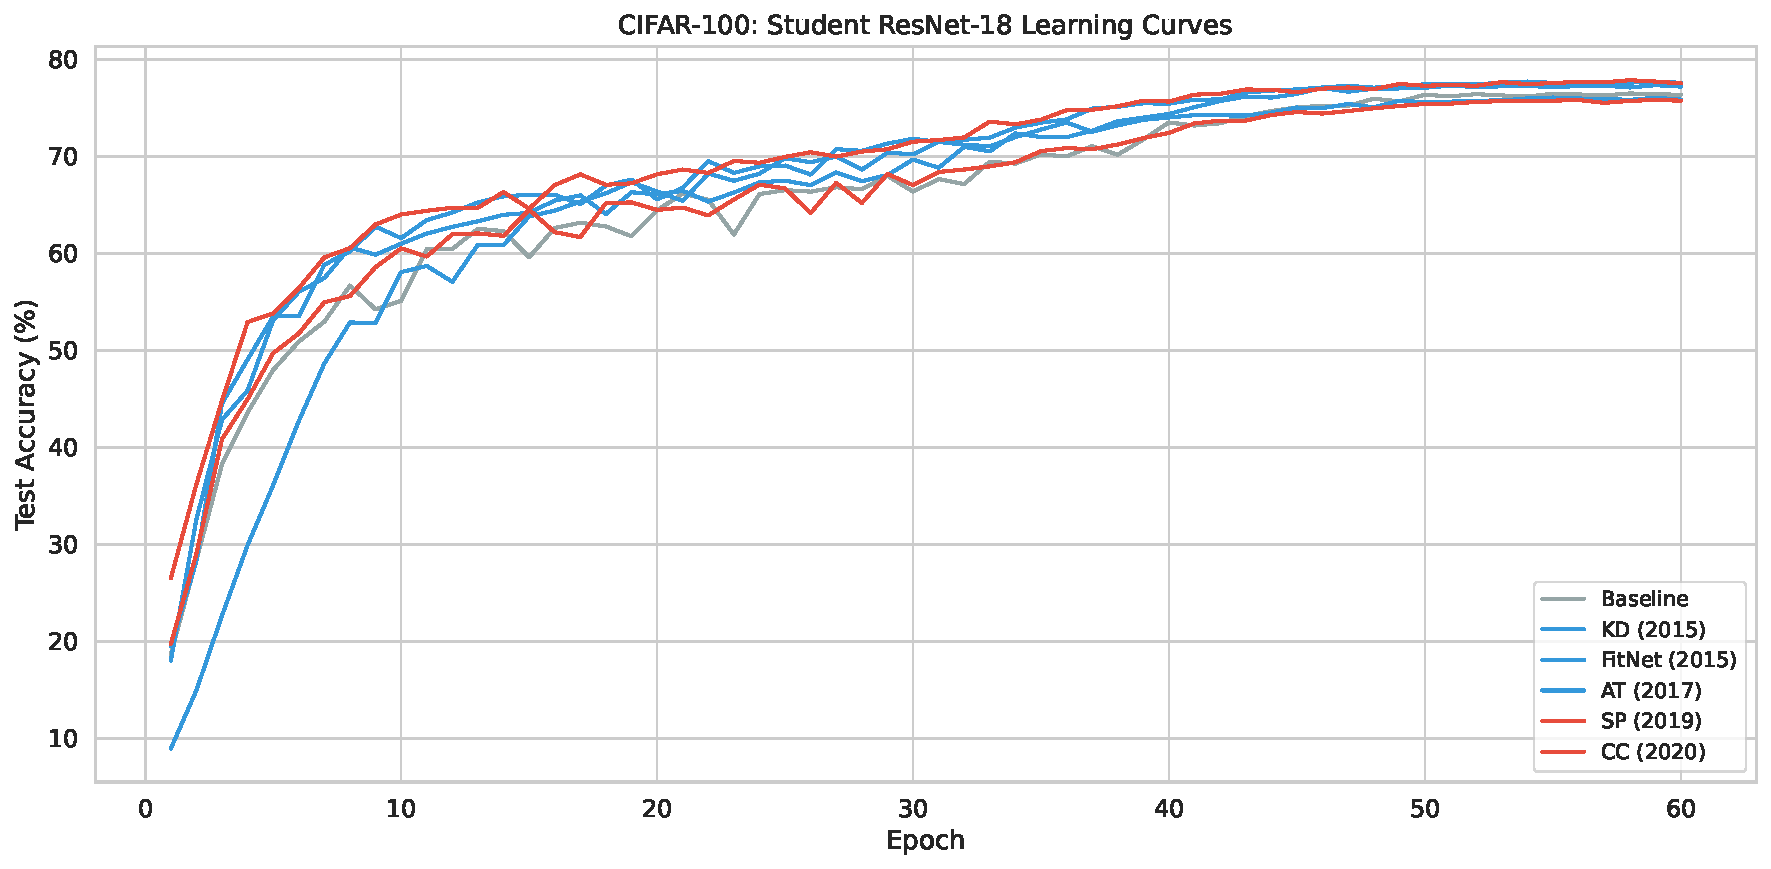
\includegraphics[width=12.0cm]{figures/learning_curves.pdf}
\caption{Test accuracy vs.\ training epoch for all KD methods.\label{fig:curves}}
\end{figure}

\begin{figure}[H]
\centering
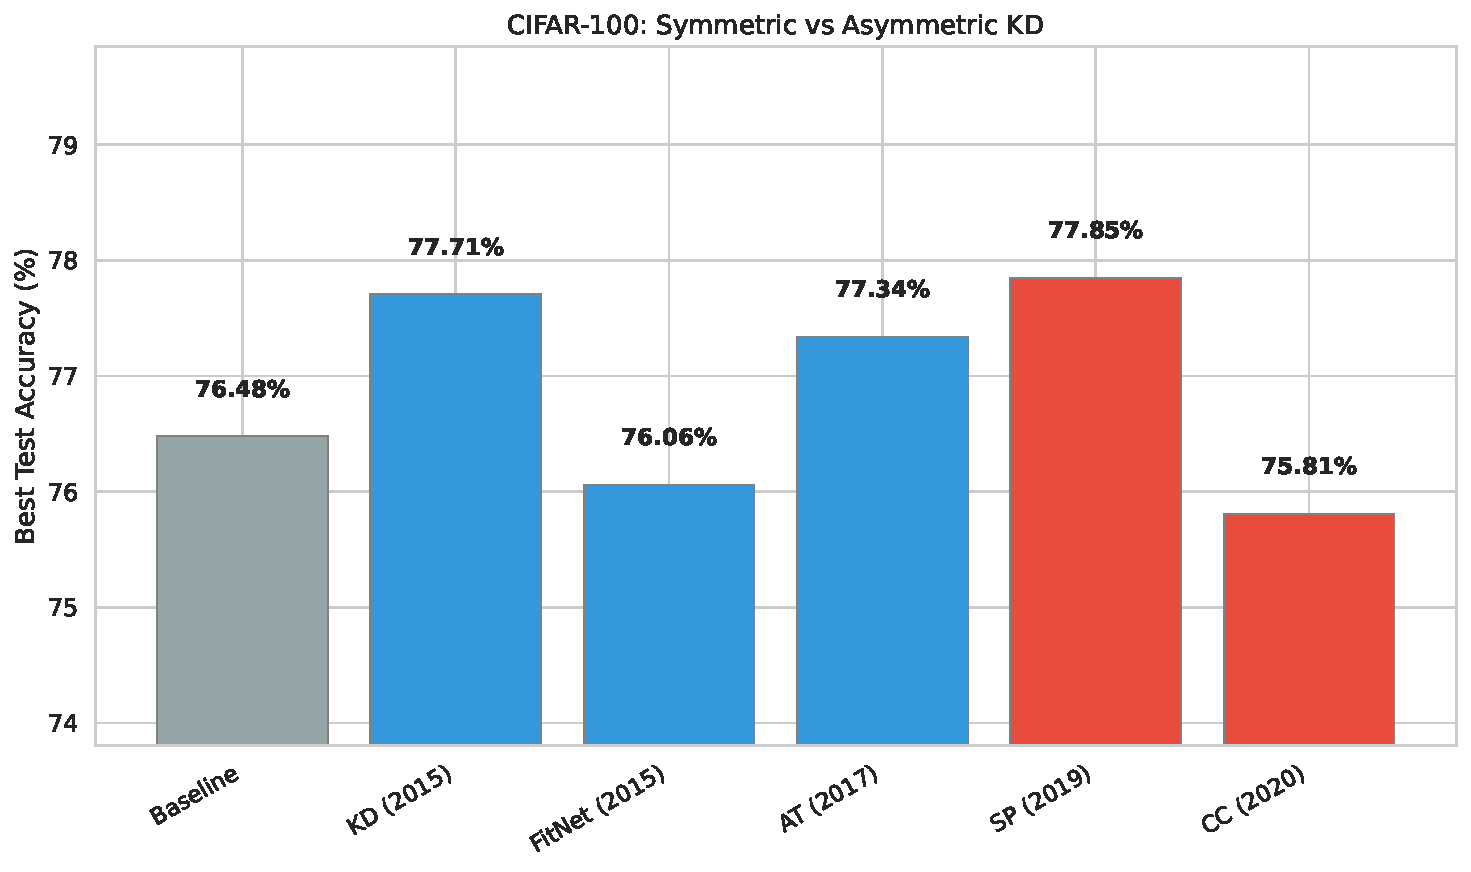
\includegraphics[width=12.0cm]{figures/bar_comparison.pdf}
\caption{Bar chart comparing best test accuracy across methods.\label{fig:bar}}
\end{figure}

\begin{figure}[H]
\centering
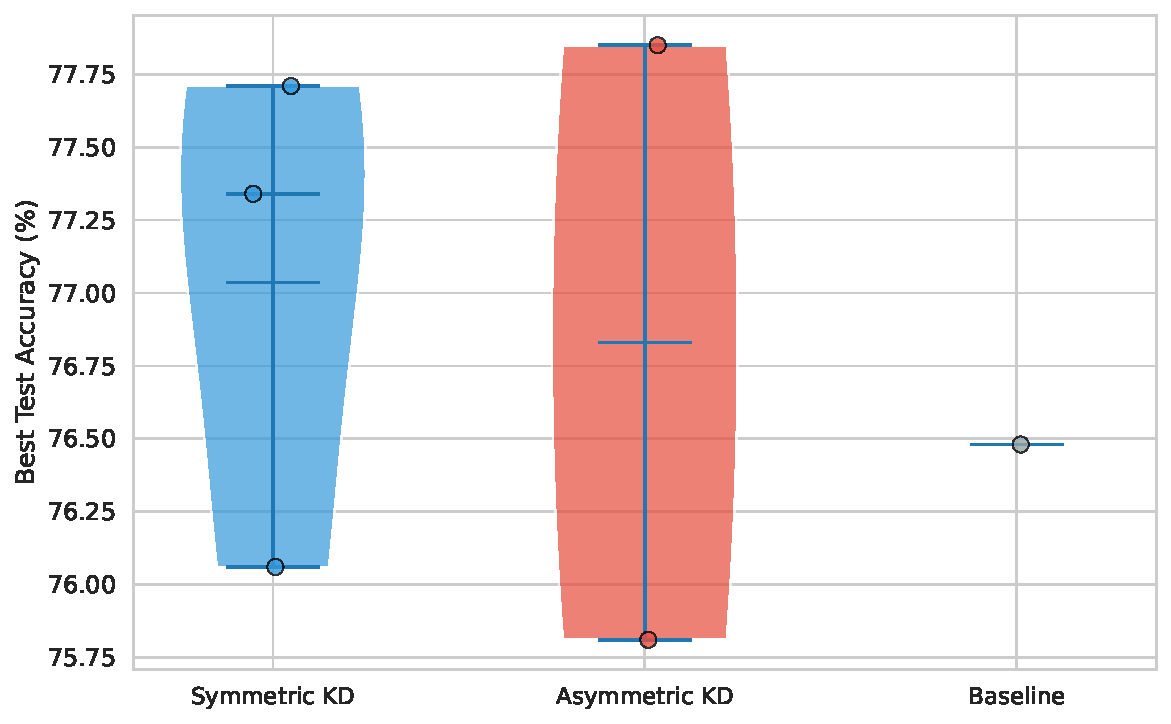
\includegraphics[width=10.0cm]{figures/category_comparison.pdf}
\caption{Violin plot of accuracy distribution by category.\label{fig:violin}}
\end{figure}

\subsection{Category Comparison}

Symmetric average: 77.04\% (range: 76.06--77.71\%). Asymmetric average: 76.70\% (range: 75.81--77.85\%). Symmetric methods show a tighter range (1.65 pp vs.~2.04 pp), suggesting more robust and predictable improvements.

\section{Discussion}
\label{sec:discussion}

\subsection{Equivariance, Invariance, and the Symmetry Spectrum}

The symmetric/asymmetric distinction can be formalized through two complementary geometric properties:

- \textbf{Symmetric KD enforces equivariance.} The student's feature map is trained to respond to input transformations in a way that is directly comparable to the teacher's response. Formally, for a transformation $g$ acting on the input, symmetric KD encourages $f_S(g(x)) \approx g(f_T(x))$ in representation space.
- \textbf{Asymmetric KD preserves invariance.} Relational structures among samples should be invariant under the mapping from teacher to student. Formally, $\mathcal{R}(f_S(x_i), f_S(x_j)) \approx \mathcal{R}(f_T(x_i), f_T(x_j))$ regardless of how individual features transform.

This equivariance/invariance framing connects our taxonomy to geometric deep learning~\cite{ref14} and clarifies the trade-off: equivariance provides stronger per-sample supervision (explaining faster convergence) but may force the student to emulate representations beyond its capacity; invariance preserves structural knowledge while allowing representational flexibility.

The taxonomy represents a spectrum rather than a strict dichotomy. \textbf{Attention Transfer} computes attention maps through spatial aggregation (relational operation) but aligns them directly (symmetric loss). \textbf{FitNet} uses a learned regression function, introducing an asymmetric component. \textbf{KD with temperature scaling} transforms distributions before comparison, emphasizing relative relationships.

\subsection{What the Taxonomy Does and Does Not Tell Us}

The symmetric/asymmetric lens provides:
- A unified vocabulary for discussing representation alignment vs.\ structure preservation
- A connection to established geometric deep learning concepts (equivariance/invariance)
- An organizing principle for understanding convergence behavior

It does not provide:
- Quantitative predictions about which method will perform best on a new dataset
- A guarantee that symmetric methods always converge faster (this is dataset-dependent)
- A replacement for existing taxonomies (output-level vs.\ feature-level, etc.)---it is complementary

\subsection{Efficiency Considerations}

Training time varies substantially across methods (Table~\ref{tab:efficiency}). RKD incurs a 41\% overhead due to pairwise distance computation ($O(b^2 d)$ per batch), while other methods add modest overhead (7--9 min over baseline). SP achieves the best accuracy at no additional computational cost over other KD methods, making it the most efficient choice in this comparison.

\subsection{Limitations}

(1) Single dataset (CIFAR-100) and architecture family (ResNet). (2) Single-run experiments per method---results should be interpreted with appropriate caution. (3) Hyperparameters adopted from prior literature without per-method tuning. (4) Limited method coverage (six of many available KD approaches). (5) The taxonomy is descriptive rather than predictive; it organizes known behaviors but does not guarantee generalization to unseen settings.

\section{Conclusions}

We introduced a symmetry-based perspective for understanding knowledge distillation methods, categorizing them as symmetric (direct alignment, enforcing equivariance) or asymmetric (relational preservation, enforcing invariance). Our experimental comparison on CIFAR-100 with six KD methods reveals that symmetric methods converge faster while asymmetric methods achieve competitive peak performance, with SP achieving the best accuracy--efficiency trade-off (77.85\%, 22 min). The taxonomy is complementary to existing classifications and is best understood as a spectrum rather than a dichotomy. We identify important limitations: single-dataset evaluation, single-run experiments, and the descriptive (rather than predictive) nature of the framework. This work provides practitioners with a conceptual tool for understanding KD method behavior and identifies directions for more rigorous comparative research.

\authorcontributions{Conceptualization, D.P. and H.Y.; methodology, H.Y.; software, H.Y.; validation, D.P.; formal analysis, H.Y.; investigation, H.Y.; resources, D.P.; data curation, H.Y.; writing---original draft preparation, H.Y.; writing---review and editing, D.P.; visualization, H.Y.; supervision, D.P.; project administration, D.P.; funding acquisition, D.P. All authors have read and agreed to the published version of the manuscript.}

\funding{This research was funded by the Guangdong Province Undergraduate Teaching Quality and Teaching Reform Project (grant no. Yue-Jiao-Gao-Han [2024] No. 30), the Guangdong Provincial Department of Education Provincial First-class Undergraduate Course (grant no. Yue-Jiao-Gao-Han [2023] No. 33), and the Shaoguan University Institutional Quality Engineering Project (grant no. Shao-Yuan-Jiao [2023] No. 30).}

\institutionalreview{Not applicable.}

\informedconsent{Not applicable.}

\dataavailability{The CIFAR-100 dataset is publicly available at \url{https://www.cs.toronto.edu/~kriz/cifar.html}. Code will be released upon publication.}

\acknowledgments{The authors acknowledge the providers of the CIFAR-100 dataset and the computational resources provided by the NVIDIA RTX 3090 GPU.}

\conflictsofinterest{The authors declare no conflicts of interest.}

\abbreviations{Abbreviations}{
\noindent
\begin{tabular}{@{}ll}
KD & Knowledge Distillation\\
AT & Attention Transfer\\
SP & Similarity Preserving\\
CC & Correlation Congruence\\
RKD & Relational Knowledge Distillation\\
KL & Kullback--Leibler divergence\\
CNN & Convolutional Neural Network
\end{tabular}}

\reftitle{References}
\begin{thebibliography}{20}
\bibitem{ref1} He, K.; Zhang, X.; Ren, S.; Sun, J. Deep residual learning for image recognition. In \textit{Proceedings of the IEEE Conference on Computer Vision and Pattern Recognition}, 2016; pp.~770--778.
\bibitem{ref2} Huang, G.; Liu, Z.; Van Der Maaten, L.; Weinberger, K.Q. Densely connected convolutional networks. In \textit{Proceedings of the IEEE Conference on Computer Vision and Pattern Recognition}, 2017; pp.~4700--4708.
\bibitem{ref3} Tan, M.; Le, Q.V. EfficientNet: Rethinking model scaling for convolutional neural networks. In \textit{International Conference on Machine Learning}, PMLR, 2019; pp.~6105--6114.
\bibitem{ref4} Cheng, Y.; Wang, D.; Zhou, P.; Zhang, T. A survey of model compression and acceleration for deep neural networks. \textit{arXiv preprint arXiv:1710.09282}, 2017.
\bibitem{ref5} Han, S.; Pool, J.; Tran, J.; Dally, W. Learning both weights and connections for efficient neural network. In \textit{Advances in Neural Information Processing Systems}, 2015; pp.~1135--1143.
\bibitem{ref6} Jacob, B.; Kligys, S.; Chen, B.; Zhu, M.; Tang, M.; Howard, A.; Adam, H.; Kalenichenko, D. Quantization and training of neural networks for efficient integer-arithmetic-only inference. In \textit{Proceedings of the IEEE Conference on Computer Vision and Pattern Recognition}, 2018; pp.~2704--2713.
\bibitem{ref7} Hinton, G.; Vinyals, O.; Dean, J. Distilling the knowledge in a neural network. \textit{arXiv preprint arXiv:1503.02531}, 2015.
\bibitem{ref8} Romero, A.; Ballas, N.; Kahou, S.E.; Chassang, A.; Gatta, C.; Bengio, Y. FitNets: Hints for thin deep nets. \textit{arXiv preprint arXiv:1412.6550}, 2014.
\bibitem{ref9} Zagoruyko, S.; Komodakis, N. Paying more attention to attention: Improving the performance of convolutional neural networks via attention transfer. \textit{arXiv preprint arXiv:1612.03928}, 2016.
\bibitem{ref10} Tung, F.; Mori, G. Similarity-preserving knowledge distillation. In \textit{Proceedings of the IEEE/CVF International Conference on Computer Vision}, 2019; pp.~1365--1374.
\bibitem{ref11} Peng, B.; Jin, X.; Liu, J.; Li, D.; Wu, Y.; Liu, Y.; Zhou, S.; Zhang, Z. Correlation congruence for knowledge distillation. In \textit{Proceedings of the IEEE/CVF International Conference on Computer Vision}, 2019; pp.~5007--5016.
\bibitem{ref12} Park, W.; Kim, D.; Lu, Y.; Cho, M. Relational knowledge distillation. In \textit{Proceedings of the IEEE/CVF Conference on Computer Vision and Pattern Recognition}, 2019; pp.~3967--3976.
\bibitem{ref13} LeCun, Y.; Bottou, L.; Bengio, Y.; Haffner, P. Gradient-based learning applied to document recognition. \textit{Proceedings of the IEEE} \textbf{1998}, \textit{86}, 2278--2324.
\bibitem{ref14} Cohen, T.; Welling, M. Group equivariant convolutional networks. In \textit{International Conference on Machine Learning}, PMLR, 2016; pp.~2990--2999.
\bibitem{ref15} Vaswani, A.; Shazeer, N.; Parmar, N.; Uszkoreit, J.; Jones, L.; Gomez, A.N.; Kaiser, \L.; Polosukhin, I. Attention is all you need. In \textit{Advances in Neural Information Processing Systems}, 2017; pp.~5998--6008.
\bibitem{ref16} Chen, X.; He, K. Exploring simple siamese representation learning. In \textit{Proceedings of the IEEE/CVF Conference on Computer Vision and Pattern Recognition}, 2021; pp.~15750--15758.
\bibitem{ref17} Grill, J.B.; Strub, F.; Altch\'{e}, F.; Tallec, C.; Richemond, P.H.; Buchatskaya, E.; Doersch, C.; Avila Pires, B.; Guo, Z.D.; others. Bootstrap your own latent: A new approach to self-supervised learning. In \textit{Advances in Neural Information Processing Systems}, 2020; pp.~21271--21284.
\bibitem{ref18} Tian, Y.; Krishnan, D.; Isola, P. Contrastive representation distillation. \textit{arXiv preprint arXiv:1910.10699}, 2019.
\bibitem{ref19} Krizhevsky, A.; Hinton, G. Learning multiple layers of features from tiny images. \textit{Technical Report}, University of Toronto, 2009.
\bibitem{ref20} Loshchilov, I.; Hutter, F. SGDR: Stochastic gradient descent with warm restarts. \textit{arXiv preprint arXiv:1608.03983}, 2016.
\end{thebibliography}

\PublishersNote{}

\end{document}
